This menu provides functions of computing and visualizing influence according to a simple model describe in ~\ref{Influence_fade_model}). Before using these functions some parameters must be input as weight of edges and influence reach.

\subsection{Select Sub-network from Sources to Targets}
\textbf{Plugins$\Rightarrow$BiNoM 2.1$\Rightarrow$BiNoM fade Influence$\Rightarrow$Select Sub-Network From Sources to Targets}\\
This function selects nodes and edges in the network between a list of sources and a list of targets.  Loops are included in the selection. For all nodes as sources or targets: select the first node and type shift+control+end.

\subsection{Update Influence Attribute}
\textbf{Plugins$\Rightarrow$BiNoM 2.1$\Rightarrow$BiNoM fade Influence$\Rightarrow$Update Weigth Influence Attribute}\\
A weight of influence as edge attribute must be affected to every edge. This dialog updates the weight attribute by selecting an  attribute et affecting their values to activation (weight=+1) and inhibition (weight=-1), 3 possible values for attribute. Generally, the attribute is "interaction" and the values "activation" or "inhibition". Be careful of lower-case and upper-case (see~\ref{Weight_Attribute_Dialog}).

\begin{figure}
\centering
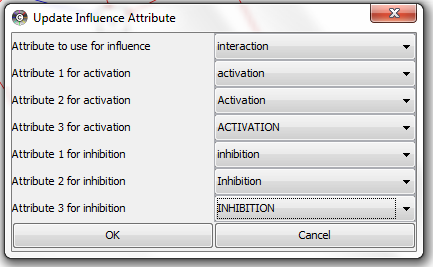
\includegraphics[width=0.7\textwidth]{graphics/Weight_Attribute_Dialog}
\caption{Dialog updating weight attribute from an other attribute}
\label{Weight_Attribute_Dialog}
\end{figure}

\subsection{Input Reach Parameter}
\textbf{Plugins$\Rightarrow$BiNoM 2.1$\Rightarrow$BiNoM fade Influence$\Rightarrow$Input Reach Parameter}\\
Input the number of paths beyond which the influence is insignificant, less than 5\%. It a real number.

\subsection{Display Network and Parameter Features}
\textbf{Plugins$\Rightarrow$BiNoM 2.1$\Rightarrow$BiNoM fade Influence$\Rightarrow$Display Network and Parameter Features}\\
Display in a text box: size of network, reach parameter, min, max and mean influence. Useful to insure the realistic value of reach.

\subsection{Display Influence Array As Text}
\textbf{Plugins$\Rightarrow$BiNoM 2.1$\Rightarrow$BiNoM fade Influence$\Rightarrow$Display Influence Array As Text}\\
The influence matrix is displayed in a text box which can be copied in the clipboard and paste in a spreadsheet, sources in columns, targets in rows, names in alphabetical order. Parameters are in title.\\\\
Text window with 2 options: 
\begin{itemize}
\item for visualizing, "nc" = not connected, only 3 digits after point for numbers,
\item for computing,  all values are numeric with all possible digits,
\end{itemize}
Same dialog as "Select Sub-network from Sources to Targets". Furthermore, structural sources and targets are preselected (respectively in degree=0, out degree=0).

\subsection{Display Influence Array as Paved Window}
\textbf{Plugins$\Rightarrow$BiNoM 2.1$\Rightarrow$BiNoM fade Influence$\Rightarrow$Display Influence Array as Paved Window}\\
Same computing as "Display Influence Array As Text". Results are in:
\begin{itemize}
\item paved window with 2 options: 
\begin{itemize}
\item activated in red, inhibited in green, light to dark according to the value, not connected in black,
\item activated in red, inhibited in blue, light to dark according to the value, not connected in white (see~\ref{paved_window}),
\end{itemize}
\item text window where are displayed details of selected area in paved window.
\end{itemize}

\begin{figure}
\centering
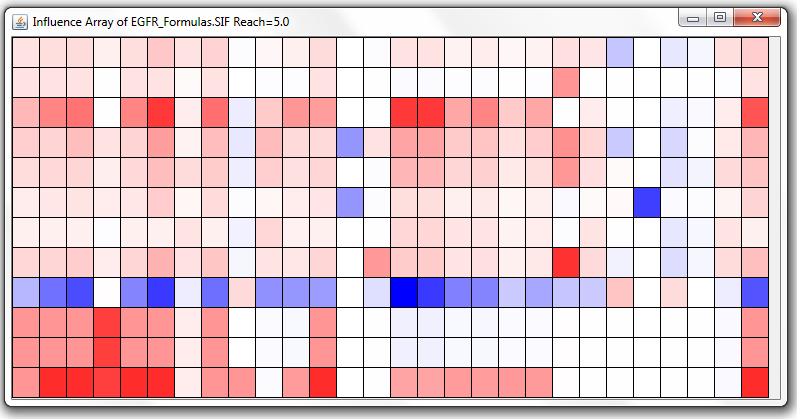
\includegraphics[width=1.0\textwidth]{graphics/paved_window}
\caption{Window paved by the level of influence between species}
\label{paved_window}
\end{figure}

\subsection{Influence by Active Nodes as Attribute}
\textbf{Plugins$\Rightarrow$BiNoM 2.1$\Rightarrow$BiNoM fade Influence$\Rightarrow$Influence by Active Nodes as Attribute}\\
Activity levels of nodes are input in an attribute "ACTIV\_IN". The result of the multiplication of influence matrix by activity level input is "ACTIV\_OUT" attribute.

\subsection{Display Influence Reach Area in Array}
\textbf{Plugins$\Rightarrow$BiNoM 2.1$\Rightarrow$BiNoM fade Influence$\Rightarrow$Display Influence Reach Area in Array}\\
Computing as "Display Influence Array for Computing" with all weights=1. Useful to appreciate the absolute level of influence by a species to other species.

\subsection{Influence Reach Area as Attribute}
\textbf{Plugins$\Rightarrow$BiNoM 2.1$\Rightarrow$BiNoM fade Influence$\Rightarrow$Influence Reach Area as Attribut}\\
Computing from selected nodes with all weights=1. Absolute influence levels are put in attribute "INFLUENCE\_AREA\_N" where N keeps every successive results. Start nodes must be noted manually. Useful to visualize the influence of a group of species.
